\documentclass{article}
\usepackage{amsmath}
\usepackage{graphicx}
\usepackage{listings}

\begin{document}

\section*{PROBLEM STATEMENT}
To implement 2D scaling transformation using OpenGL in C and to draw and scale a polygon against a defined coordinate system. The program will also draw the coordinate axes for better visualization.

\section*{THEORY}
2D scaling is a geometric transformation that alters the size of an object. Scaling can either magnify (enlarge) or minify (shrink) the object. It is defined by two scaling factors, \(s_x\) and \(s_y\), which scale the object along the x-axis and y-axis respectively.

The scaling transformation matrix is given by:
\[
S = \begin{bmatrix}
s_x & 0 \\
0 & s_y
\end{bmatrix}
\]

When a point \((x, y)\) is scaled, the new coordinates \((x', y')\) are computed as:
\[
x' = s_x \cdot x
\]
\[
y' = s_y \cdot y
\]

\section*{ALGORITHM}

\begin{enumerate}
    \item Initialize the coordinates of the polygon vertices.
    \item Draw the coordinate axes using the Bresenham line drawing algorithm.
    \item Draw the original polygon.
    \item Apply the scaling transformation to each vertex of the polygon.
    \item Draw the scaled polygon in a different color.
\end{enumerate}

\section*{FLOWCHART}
\begin{center}
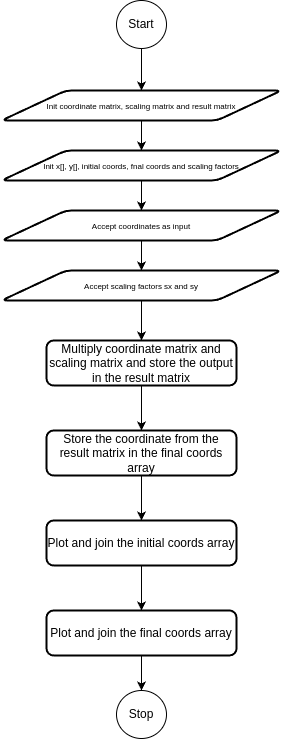
\includegraphics[width=0.7\textwidth]{flowchart.png}
\end{center}

\section*{SAMPLE I/O}
\textbf{Input:}
\begin{verbatim}
Polygon vertices: (10, 10), (200, 10), (200, 200), (10, 200)
Scaling factors: sx = 0.5, sy = 0.5
\end{verbatim}

\textbf{Output:}
The original and scaled polygons are displayed in a window with coordinate axes.

\section*{DISCUSSIONS}
\begin{itemize}
    \item \textbf{Advantages}: Scaling is a straightforward transformation that is easy to implement and visualize. It is useful in various applications such as resizing images and models.
    \item \textbf{Disadvantages}: Uniform scaling (same factor for both axes) preserves the shape of the object, but non-uniform scaling (different factors for each axis) can distort the object.
    \item \textbf{Applications}: Scaling is widely used in graphics, animation, CAD software, and game development for resizing objects and models.
\end{itemize}

\section*{CONCLUSION}
The 2D scaling transformation is fundamental in computer graphics for resizing objects. Implementing this transformation using OpenGL provides a visual understanding of how scaling affects the size and shape of a polygon. Drawing coordinate axes helps in better visualization of the transformation effects.


\end{document}
